
\vsp
\section{ \auspice\ design \& implementation}
\label{sec:design}

In this section, we present the design and implementation of \auspice, a massively scalable global name service designed for high mobility. We begin by describing how the envisioned service enables endpoint mobility, and the design requirements in order to realize that vision.


\begin{figure}[htbp]
\begin{center}
\vspace{-0.1in}
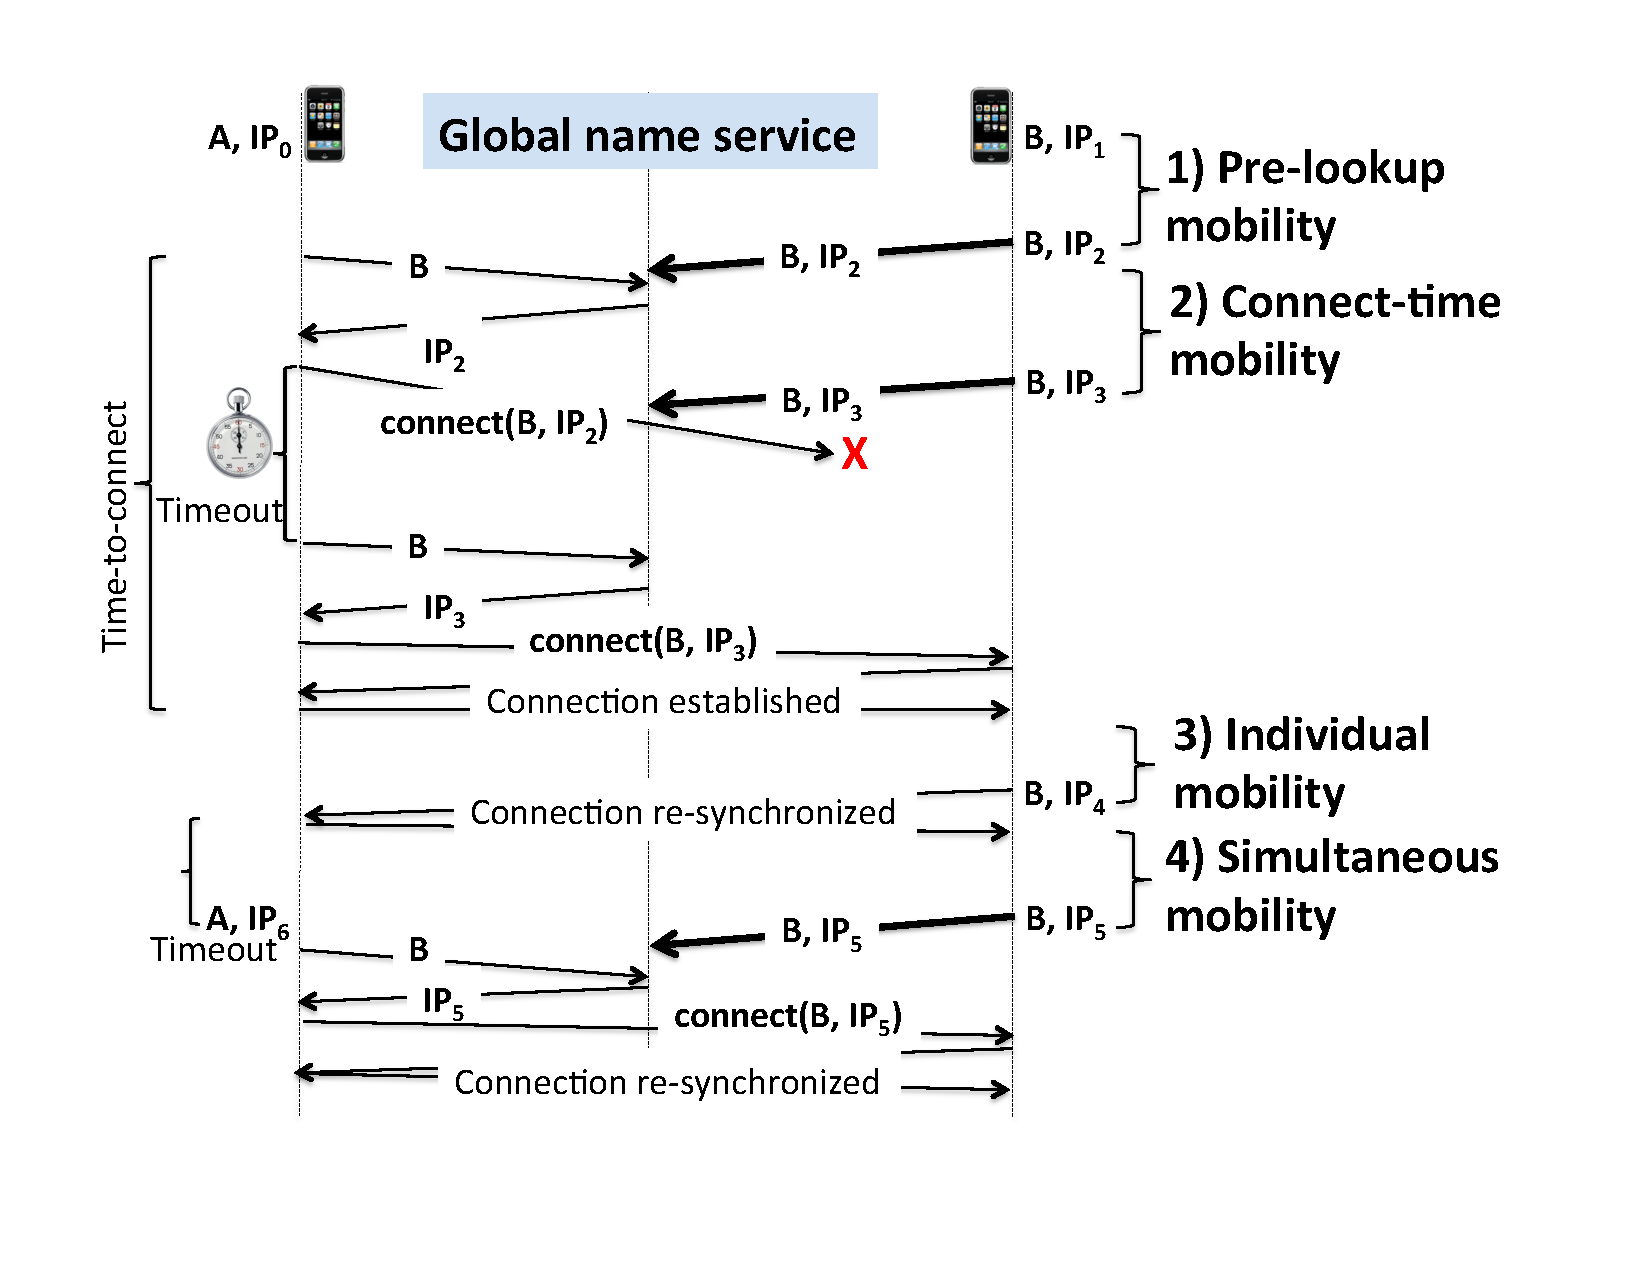
\includegraphics[scale=0.3]{auspice/figure/4mobility.pdf}
\vspace{-0.5in}
\caption{Four kinds of mobility---(1) Pre-lookup, (2) Connect-time, (3) Individual, (4) Simultaneous---three of which require a global name service.} 
\vspace{-0.3in}
\label{fig:4mobility}
\end{center}
\end{figure}

%\para{How GNS enables mobility}
{The GNS works to enable endpoint mobility as shown in Figure \ref{fig:4mobility}. An endpoint A initiates communication with another endpoint B by querying the GNS for B's current addresses and connecting to one of them, thereby enabling pre-lookup mobility. If B moves after A's query but before before a connection has been mutually established through a three-way handshake (connect-time mobility), A times out and reverts back to the GNS. After a connection has been established, if either endpoint moves one at a time (individual mobility), it can re-synchronize the connection with a bilateral three-way handshake without relying upon the GNS (noting however that router-level late-binding proposals relying on a GNS-like infrastructure have also been proposed \cite{serval,MobilityFirst-UMASS}). If an endpoint moves mid-connection after the other endpoint has moved but before it could re-synchronize the connection (simultaneous mobility), one or both endpoint(s) eventually query the GNS and re-synchronize the connection.}



\subsection{Design goals}\vsp
\label{sec:design_goals}

\begin{figure}[htbp]
\begin{center}
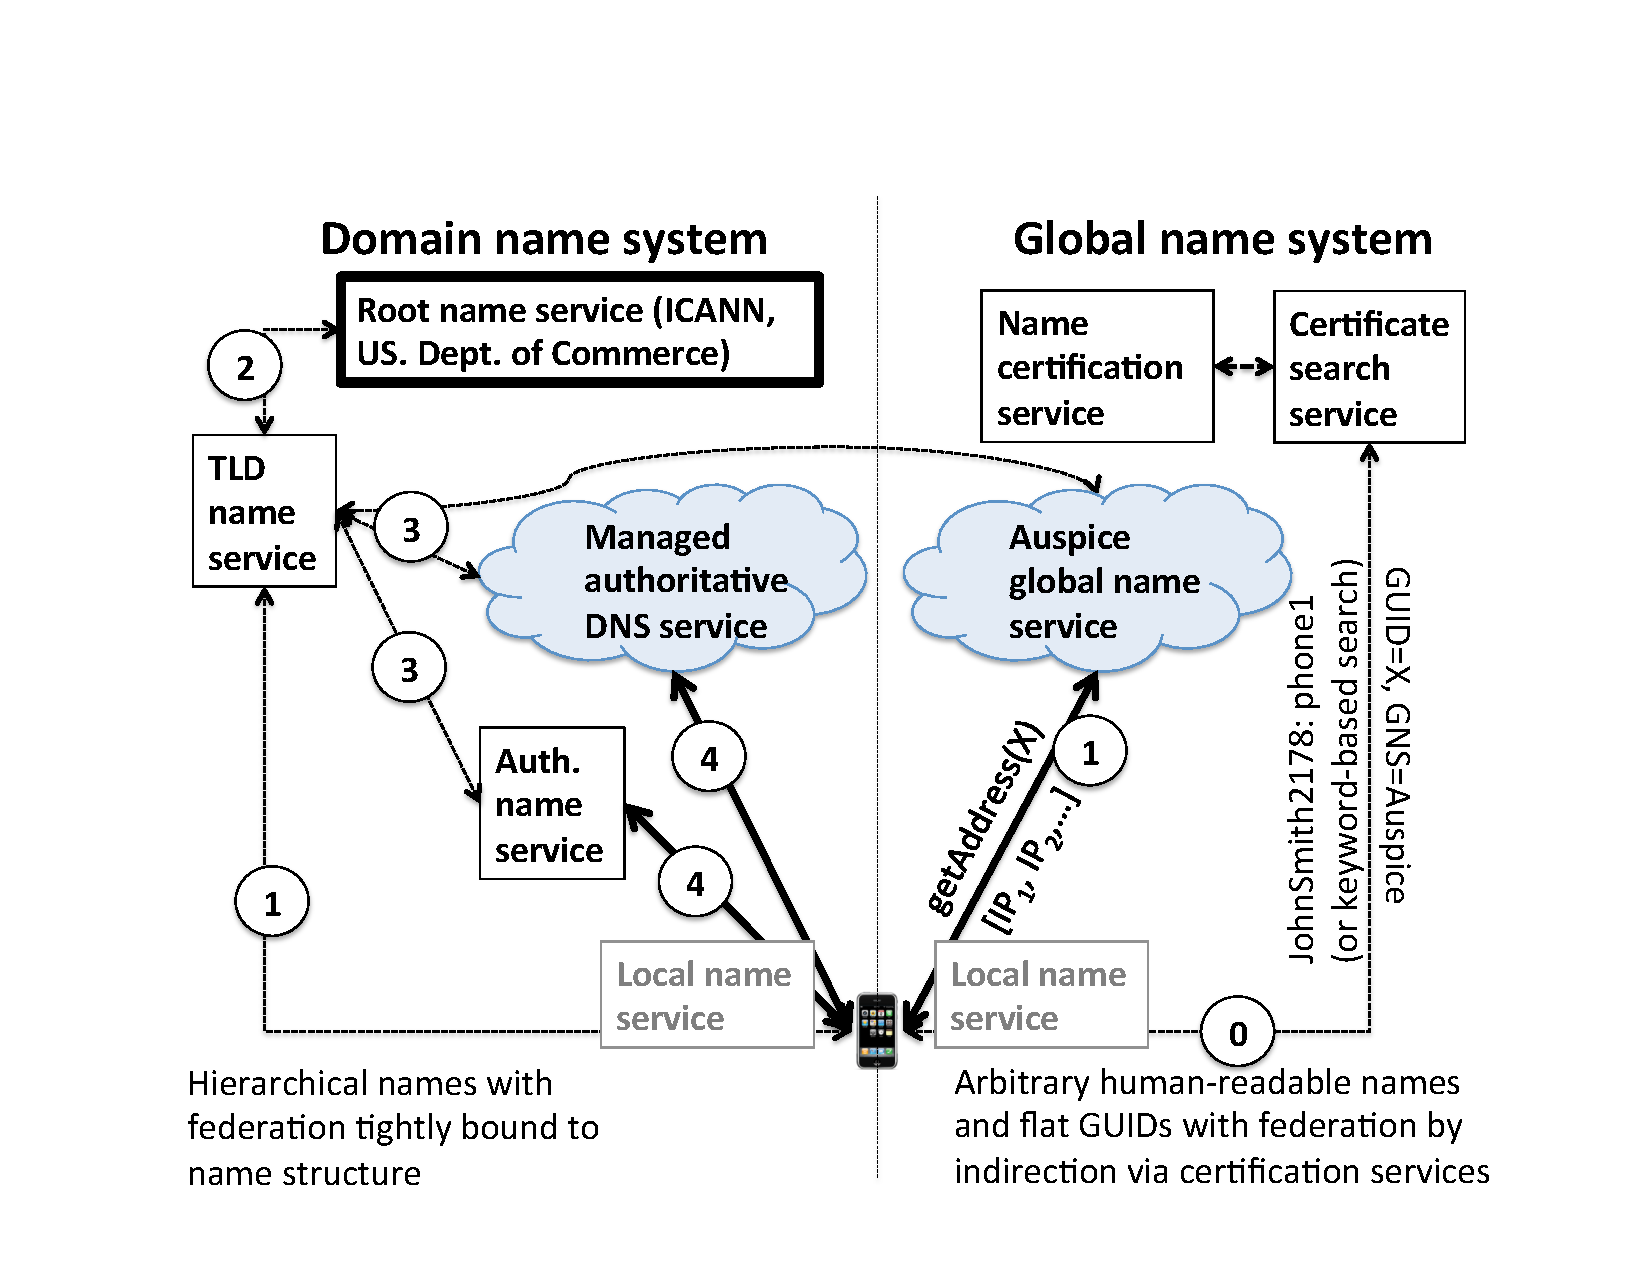
\includegraphics[scale=0.25]{auspice/figure/DNS-GNS.pdf}
\caption{\small{DNS vs. GNS: Auspice can be deployed as a managed DNS provider today (left) or as a GNS provider that provides resolution service for its customer GUIDs (right). Name certification services (say Verisign) bind a human-readable name to a GUID and its GNS provider, and certificate search services (say Google) can help index and distribute certificates from all certification services. Solid (dotted) lines represent frequent (infrequent) query paths for a given mobile destination. Except for the tightly controlled DNS root  service, all services above are designed to be purveyed competitively.} 
}\label{fig:DNS_GNS}
\end{center}
\end{figure}

 
 A GNS as above must meet the following design goals.

{\bf (1) Time-to-connect performance}: The design must ensure low latencies  for name lookups to return up-to-date values (which determines the {\em time to connect} to a destination when the value being queried for is an address like above).  An implicit goal here is to not only support use-cases like above but also to enable other architectural proposals that involve routers late-binding names to addresses near the destination \cite{serval,MobilityFirst-UMASS}; enabling seamless mid-connection mobility \cite{Migrate,ECCP}, etc., so that any endpoint or router gets the feel of the lookup service being located tens of milliseconds away.

{\bf (2) Resource cost}: The design must ensure low replication cost. A naive way to minimize lookup latencies is to replicate every name record at every available location, however high mobility implies high update rates, so the cost of pushing each update to every replica would be prohibitive. Worse, load hotspots can actually degrade lookup latencies  instead of improving them.

{\bf (3) High availability}: The design must be resilient to failures of nodes including disasters impacting an entire datacenter or stub network. By consequence, the design must also prevent crippling load hotspots.

%{\bf (4) Consistency}: The system must achieve the above objectives while ensuring flexible consistency semantics for name records as specified by their owners. A naive way to achieve the first two goals is to use aggressive caching with large TTLs, clearly an unusable scheme in mobile scenarios as inconsistency implies unreachability.

{\bf (4) Security}: The design must be robust to malicious user behavior such as hijacking or corrupting name records. The design must support flexible access control policies to ensure the desired privacy of name records.

{\bf (5) Federation}: The design must allow different name service providers to co-exist and for users to freely choose their preferred provider, and must be easily deployable in today's Internet.

{\bf (6) Extensibility}: The design must be extensible to supporting a rich set of attributes associated with a name and policies for dealing with mobility, multihoming (e.g.,``prefer WiFi to cellular''), etc. The design should be agnostic to how names, addresses, and resolution policies are represented by a future Internet architecture.

Note that ``scalability'' is not an explicitly defined goal above because it is subsumed by the first three goals, i.e., a design maximizing performance and availability for any given resource cost is implicitly designed to improve the former with commensurately more resource expenditure. We explicitly quantify this tradeoff in $\S$\ref{sec:scalability}.


%Figure \ref{fig:4mobility} illustrates the four kinds of mobility and shows how the GNS helps handle three of these---pre-lookup, connect-time, and simultaneous mobility. Only individual connection mobility can be handled bilaterally without the GNS (although router-level late-binding proposals relying on a GNS-like infrastructure have also been proposed \cite{serval,MobilityFirst-UMASS}). In addition to emphasizing the importance of the GNS for handling mobility, the figure also reinforces the first four of the six design goals laid out above. 



\subsection{Design overview}


To address the above goals, \auspice\ is designed as a massively geo-distributed key-value store that performs name resolution. The geo-distribution is essential to the latency and availability goals while the key-value design enables extensibility. Each {\em name record} in \auspice\ is associated with a globally unique identifier (GUID) that is also the record's primary key. A name record contains an associative array of key-value pairs as shown, wherein each key $K_i$ is a string and the value $V_i$ may be a string, a primitive type, or recursively a key-value pair.

GUID  $\ | \ K_1, V_1 \ | \ K_2, V_2 \ \ | \cdots $

The GUID is a self-certifying identifier determined as a compact hash of a public key. Each name record is associated with a globally unique human-readable aliases that are bound to the GUID by a certificate supplied by one or more {\em name certification service(s)} (NCS). Loosely speaking, the human-readable alias is analogous to a DNS domain name and a name record to a zone file, but with the following important differences.

{\bf{Security.}} As shown in Fig. \ref{fig:DNS_GNS}, to initiate communication with a destination Y, an endpoint X must first obtain a certificate of the form $[\textit{JohnSmith1956:Phone1}, Y, P]_{K^-}$ that binds the human-readable alias to the GUID Y and its GNS provider P, and is signed by the private key $K^-$ of an NCS that X trusts. A certificate search service can help index certificates from different NCSes, and help X find a certificate from a trusted NCS as well as find the human-readable alias based on keyword searches. 

{\bf{Federation.}} Unlike ICANN and root DNS servers that respectively act as a single name adjudication authority and root of trust, the design above decentralizes trust across different NCS providers and potentially allows for endpoints to use quorum-based approaches to resolve name conflicts (or conflicting certificates). More importantly, the federated design above allows for endpoints to select arbitrary human-readable names and NCS providers unlike DNS that restricts domain names to be hierarchical and federation and the DNSSEC keychain to strictly follow the name structure. An inevitable downside of the above design is that two endpoints can only communicate securely if they share a trusted NCS provider, a tradeoff we argue is preferable to the single root of trust model that some perceive as arbitrary \cite{ICANN-debate-Sems,ICANN-debate-Gross}. 

{\bf{Extensibility.}} The design above cleanly separates the GNS provider's resource-intensive responsibility of name resolution under high mobility from the slow-changing certification process. It also allows for the GNS provider to be deployed today as a managed authoritative DNS provider (Fig. \ref{fig:DNS_GNS}) with the DNSSEC key deriving the GUID. Finally, the key-value store API enables an extensible name record representation. By default, each top-level key has associated read and write ACLs that could either be a blacklist or whitelist of GUIDs that respectively have read or write access. For example, a name record that helps context-aware delivery and multihoming policies (as detailed in $\S$\ref{sec:context}) is below.
\verb+{GUID+
\verb+: {[IPs:[[IP=23.55.66.43, type=Unlimited],+ \\
\verb+[IP=62.44.65.75, type=Limited]], geoloc:+\\
\verb+[[lat, long], readWL: NONE], multihome_policy:+
\verb+Unlimited]}+

%By default, all columns and network addresses in particular can be read by all but written to only using the GUID's private key. Some {\em keyword} attributes like netAddress and geoLocation have special support (unlike developer-defined attributes), for example, in order to efficiently maintain indexes for value-based reverse lookups or for non-default privacy policies like allowing only whitelisted reads for geoLocation.

%For the former, it suffices to think of a {\em name} as a domain name, a {\em name record} as the associated zone file, and a {\em name server} as analogous to a DNS name server. For ease of exposition, we assume one name server per geo-location.

\subsection{\auspice's geo-distributed design}

\begin{figure}[t]
\centering
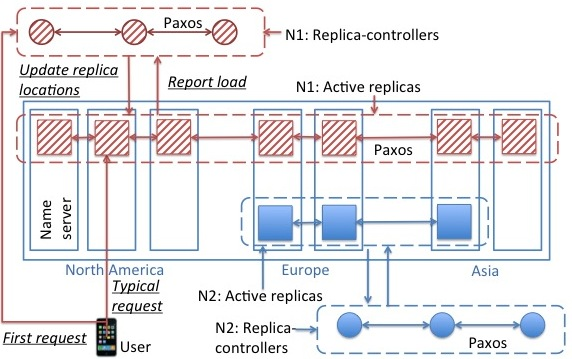
\includegraphics[scale=0.4]{auspice/gns-dns/Slide3.jpg}
\vspace{-0.2in}
\caption{Geo-distributed name servers in \auspice.  Replica-controllers  (logically separate from active replicas) decide placement of active replicas and active replicas handle requests from end-users. N1 is a globally popular name and is replicated globally; name N2 is  popular in select regions and is replicated in those regions.}
\vspace{-0.2in}
\label{fig:auspice}
\end{figure}


Next, we explain how our GNS provider \auspice\ achieves the first three goals. At the core of \auspice\ is a placement engine that achieves the latency, cost, and availability goals by adapting the number and locations of replicas of each name record in accordance with (1) the lookup and update request rates of the name, (2) the geo-distribution of requests for that name, and (3) the aggregate request load on the system across all names. 

%The key to ensuring high availability and flexible consistency is a two-tier consensus engine for each name; the first ``control'' tier infrequently recomputes and migrates the current set of replicas of each name record, and the second ``data'' tier upon each write or read coordinates with other replicas to ensure the necessary consistency semantics.% In addition to the placement algorithm, the design and implementation challenges we address include managing a very large number of parallel Paxos instances (one per name per tier); correctly changing Paxos group membership in a live system; efficiently routing client requests;  TBD\tbd{Need to say why challenging somewhere clearly}.


Figure \ref{fig:auspice} illustrates the placement engine. Each name is associated with a fixed number, $M$ (=3 default), of  \emph{replica-controllers} and a variable number of  {\em active replicas} of the corresponding name record. The number and locations of the replica-controllers is fixed and is computed using $M$ well-known consistent hash functions each of which maps the name to a name server location. The replica-controllers are responsible only for determining the number and locations of the active  replicas, and the actives replicas are responsible for keeping name records updated and responding to client's requests. The replica-controllers implement a replicated state machine using Paxos \cite{LamportPaxos} so as to maintain a consistent view of the current set of active replicas despite failures. 



%The key insight in \auspice\ is a placement engine to compute the number and locations of replicas of a name record  based on the lookup to update ratio of the name,  the geo-distribution of its demand, and the aggregate request load on the system.

%
%At an abstract level, \auspice\ design can be described as consisting of two planes: a ``control plane'' which determines the locations at which each name record is replicated, and a ``data plane''  consisting of  replicas of name records whose function is to handle address lookups and updates for end-users.  Physically, both these planes run across the set of name servers on which \auspice\ is deployed. 
%
%
%The role of the control plane for a name is handled by a fixed number, $M$, of  \emph{replica-controllers}. The number and locations of the replica-controllers is fixed and is computed using $M$ well-known consistent hash functions each of which maps the name to a name server location. The replica-controllers implement a replicated state machine using Paxos \cite{LamportPaxos} so as to maintain a consistent view of the current set of active replicas despite failures. 
%

%The control plane periodically runs a placement algorithm and places a name record based on the inferred pockets of demand for that name, the lookup-to-update ratio of the name, and the aggregate system load so as to achieve low lookup latency, low update cost, and desired level of availability. 



% achieve low response times, low update costs, and high availability.
%based on the geo-locality of demand for that name while mitigating load hotspots across all locations. 

%The key insight in \auspice\ is a placement engine to compute the number and locations of resolver replicas for a name based on the geo-locality of demand for that name while mitigating load hotspots across all locations. 

%% 'Active replicas' or  'replicas'?

%Figure \ref{fig:auspice} illustrates the architecture of \auspice.  Each name is associated with a fixed number, $M$, of  \emph{replica-controllers} and a variable number of  {\em active replicas} of the corresponding resolver. The locations of the replica-controllers is fixed and computed using $M$ well-known consistent hash functions each of which maps the name to a name server location. The replica-controllers form the ``control plane'' and are responsible only for determining the number and locations of active replicas, and the active replicas are responsible for maintaining resource records and responding to lookup and update requests. 


%

Computing the active replica locations for each name proceeds in epochs as follows. At bootstrap time, the active replicas are chosen to be physically at the same locations as the corresponding replica-controllers. In each epoch, the replica-controllers obtain from each active replica a summarized load report that contains the request rates for that name from different {\em regions} as seen by that replica. Regions could either be IP prefixes or geographic regions, e.g., cities, that partition users into non-overlapping groups so as to capture locality. Each active replica's load report consists of a spatial vector of request rates as seen by that replica. The replica-controllers aggregate these load reports to obtain a concise spatial distribution of all requests for the name.



\eat{
The replica-controllers execute Paxos to compute the placement decision in a coordinated manner for each name. During periods of graceful execution, only one replica-controller (the Paxos coordinator) actually invokes the mapping algorithm while the others simply accept its proposed placement; consensus ensures that the replica-controllers maintain a consistent view of the current set of active replicas despite failures.
}

%\begin{figure}[t]
%\begin{center}
%%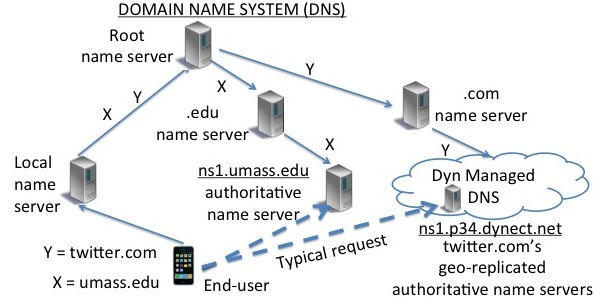
\includegraphics[width=3in, height=2.4in]{Auspice-arch/Slide1}
%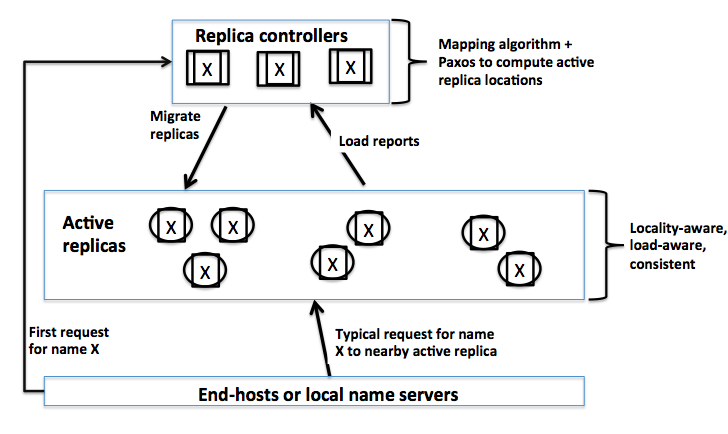
\includegraphics[width=3in]{graph/slide2SS}
%\vspace{-0.2in}
%\caption{\auspice\ design: Clients send typical requests to nearby active replicas of resolvers. Replica-controllers compute the number and locations of active replicas for each name based on load reports in each epoch.}
%\vspace{-0.2in}
%\label{fig:arch}
%\end{center}
%\end{figure}
\vsp
\subsubsection{Placement algorithm} 
\vsp
%We have also developed simple heuristic placement algorithms that are computationally efficient. A heuristic algorithm that appears promising in our ongoing evaluation is one that creates a number of active replicas proportional to the ratio of the read rate and write rate for the name; places some replicas at the locations that receive the highest number of requests for that name and places the rest at random locations; and redirects client requests to active replicas taking both round-trip network latency and name server load into account. 

In each epoch, the replica-controllers use a {placement algorithm} that takes as input the aggregated load reports and capacity constraints at name servers to determine the number and locations of active replicas for each name so as to minimize client-perceived latency. We have formalized this {\em global} optimization problem as a mixed-integer program and shown it to be computationally hard.  As our focus is on simple and efficient algorithms, we defer the details of the optimization approach to a techreport \cite{techreportAuspice}, and use it only as a benchmark in small-scale experiments against \auspice's heuristic algorithm%\tbd{Need the optimization formulation here.}.

%We have shown that the placement problem can be formulated as a mixed-integer optimization problem that is computationally hard (refer to the tech report \cite{techreportAuspice}), so we use it only as a benchmark in small-scale experiments.

\auspice's placement algorithm is a simple heuristic  and can be run {\em locally} by each replica-controller. The placement algorithm computes the number of replicas using the lookup-to-update ratio of a name in order to limit the update cost to within a small factor of the lookup cost. The number of replicas is always kept more than the minimum number needed to meet the availability objective under failures.   The location of these replicas are decided to minimize lookup latency by placing a fraction of replicas close to pockets of high demand for that name while placing the rest randomly so as to balance the potentially conflicting goals of reducing latency and balancing load among name servers.
%The location of these replicas are decided partly based on the locality of demand, while the rest of the replicas are placed randomly in order to achieve a good tradeoff between locality-awareness and load-balance. 

{
%To this end, we develop a simple heuristic placement algorithm that is computationally efficient. Our algorithm places active replicas in a  locality- and load-aware manner by leveraging three key design insights: it creates a number of active replicas proportional to the ratio of the read rate and write rate for the name; it places some replicas at the locations that receive the highest number of requests for that name and places the rest at random locations; 

%and it redirects client requests to active replicas taking both round-trip network latency and name server load into account. 

%\bp{How we compute the number of replicas}
Specifically, the placement algorithm computes the number of replicas for a name as ($M+ \beta R_i/W_i$), where $R_i$ and $W_i$ are the lookup and update rates of name $i$, $M$ is the minimum number of replicas needed to meet the availability goal (\S \ref{sec:design_goals}), and $\beta$ is a replication control parameter.  The placement algorithm dynamically adjusts $\beta$ to control the number of replicas so as to trade off latency benefits against update costs given capacity constraints as follows. In each epoch, the replica-controllers recompute $\beta$ so that the aggregate load in the system corresponds to a predetermined threshold utilization level $\mu$ ( = 0.7 default). For simplicity of exposition, suppose read and write operations impose the same load, and the total capacity across all name servers (in reads/sec) is $C$. Then, $\beta$ is set so that  
\vsp
\begin{equation}
\mu C = \sum_i R_i  + \sum_i (M + \beta  \frac{R_i}{W_i}) W_i
\label{eq:mu}
\end{equation}
\vsp
\vsp

 where the right hand side represents the total load summed across all names. The first term in the summation above is the total read load and the second is the total write load. 
%\begin{equation}
%\beta = \frac{C\mu - M \sum_i W_i}{\sum_i R_i}- 1
%\label{eq:beta}
%\end{equation}
%It is straightforward to extend the above heuristic to scenarios where read and write operations impose unequal amounts of load on a name server
 Having computed $\beta$ this equation, \auspice\ computes the locations of replicas for name $i$ as follows. Out of the $M + \beta R_i/W_i$ total replicas, a fraction, $f$ (=0.5 default), of replicas are chosen according to locality, i.e., the replica-controllers use the spatial vector of load reports to select $K = f \times(M + \beta R_i/W_i)$ name server locations that are respectively the {\em closest} to the top $K$ regions sorted by demand for name $i$. The remaining $M + \beta R_i/W_i - K$  are chosen randomly without repetition.
 
The top-K ``closest'' replicas above are chosen as the closest with respect to round-trip latency plus load-induced latency measured locally at each name server. An earlier design simply chose the top-K according to round-trip locality alone; however, we found that adding load-induced latencies in this step in addition to choosing the remaining replicas randomly ensures better load balance and results in lower overall user-perceived latency.

%Explicitly, we compute replication parameter $\beta$ in each replication epoch to make sure the total load in the system is within a certain threshold $C$. With each name $i$ having $(\alpha + \beta \times R_i/W_i)$ replicas, where $R_i$ and $W_i$ are lookup and update rates for name $i$ respectively, the total load is the sum of lookup load and update load, i.e., 
%\begin{equation}
%\sum_i R_i + \sum_i (\alpha + \beta \times \frac{R_i}{W_i}) W_i
%\end{equation}
%To make sure this load is within the threshold $C$, we can compute $\beta$ as
%\auspice\ uses the max value of $\beta$ that satisfy Eq \ref{eq:beta}.


%\bp{How we place locations of replicas}
%\auspice\ places replicas by taking into account both the geo-locality of requests and load-balancing across name servers. Replicas are selected using the votes received by a name server.  Votes for a name-server are equal to sum of requests from the geo-graphic region to which this name-server is the closest name server. The number of replicas selected based on locality is determined by the locality parameter $K$. We choose up to $K$ name servers receiving maximum number of votes as be resolvers. The remaining name servers are chosen randomly to ensure load balancing. 

}

%\vfill\eject



%\subsubsection{Sequential consistency}
%
%- Paxos group between active replicas
%
%- role of sequence numbers
%
%- changing set of active replicas
%
%\subsubsection{Adding and deleting names}
%
%\subsubsection{Handling name server failures}



\vsp
\subsubsection{Routing client requests}

\label{sec:routing_client_requests}

Next, we describe how individual requests from end-hosts are routed to a suitable name server.
The list of all name servers  is known to each name server and can be obtained by contacting any name server. 
End-hosts can either directly send requests to a name server or channel them through a local name server like today. 
When a local name server encounters a request for a name for the first time, it uses the known set of all name servers and hash functions to determine the replica-controllers for that name and sends the request to the closest replica-controller. 
The replica-controller then returns the set of active replicas for the name and the client resends the request to the closest active replica.  In practice, we expect replica-controllers to be contacted infrequently as the set of active replicas can be cached and reused. 
%Local name server requests up to three active replicas to get a response.  A timeout value is set for every request sent and the request is sent to the next closest active replica on a timeout.

%To answer lookup requests, local name servers implement a TTL-based cache to store the name records received.






%A local name server redirects end-users requests to a resolver chosen in a locality and load-aware manner. To achieve both these properties, local name servers maintain latency estimates to name servers that reflect both network latency and server-load induced latency (or server latency). Among a set of resolvers,  a local name server always redirects requests to the closest name server based on  the latency estimates. 

%A local name server in \auspice\ redirects end-users requests to a resolver chosen in a locality and load-aware manner. To achieve both these properties, local name servers maintain latency estimates to name servers that reflect both network latency and server-load induced latency (or server latency). Among a set of resolvers,  a local name server always redirects requests to the closest name server based on  the latency estimates.  Network latency estimates change slowly and therefore every local name server maintains round-trip latency estimates to all name servers using infrequent measurements. Server latency changes frequently due to dynamic workloads.  In an Internet scale deployment with tens of thousands of name servers, maintaining server latency information would add significant overhead.  Hence, server latency  is maintained only for a smaller number of frequently contacted name servers.

Network latency as well as server-load-induced latency help determine the closest active replica and the closest replica-controller at a local name server. As network latency estimates change slowly, local name servers maintain round-trip latency estimates to all name servers using infrequent pings.  To incorporate the load-induced latency, the latency estimate to a name server is passively measured as a moving average over lookups sent to that name server. The local name server also maintains a timeout value based on the moving average and variance of the estimates.  If a lookup request sent to a name server times out, the local name server infers that either the route to the server  is congested or the server is overloaded, and it increases its latency estimate to that name server by a fixed factor (=1.1 default). Overall, this method ensures that  if multiple lookups sent to a name server time out, the estimated latency becomes very high and the local name server stops sending requests to that name  server, which effectively acts as a more agile load-balancing policy in the request routing plane (complementing the replica placement plane above that operates in coarser-grained epochs).


\subsubsection{Consistency with static replication}
\label{sec:consistency}

%\tbd{Rewrite entire section.}

%The above proximity-based strategy can route both lookup (or read) and update (or write) requests for a name to any active replica. In order to ensure low lookup latency, it is important for them to be served locally from an active replica. This means that the onus of replica coordination in order to maintain any nontrivial consistency semantics falls on the update procedure. But why should we care about consistency when DNS and network protocols in general prize liveness over consistency\cite{consensus-routing}?

As a global name-to-address resolution service, \auspice\ must at least ensure the following property: {\em all active replicas must eventually return the same value of the name record and, in a single-writer scenario, this value must be the last update made by the (only) client}; ``eventually" means that there are no more updates to a name record and no replica failures for sufficiently long. Not satisfying this {eventual consistency} property means that a mobile client may be  persistently unreachable even though it is no longer changing its network address(es). 

With a static set of replicas, it is straightforward to support this property. A replica receiving  a client update need only record the write in a persistent manner locally, return a commit to the client, and lazily propagate the update to other active replicas for that record. Lazy propagation is sufficient to ensure that all replicas eventually receive every update committed at any replica, and a deterministic reconciliation policy, e.g., as in Dynamo \cite{dynamo}, suffices to ensure that concurrent updates are consistently applied across all replicas. Temporary divergence across replicas under failures can be shortened by increasing durability, i.e., by recording the update persistently at more replicas before returning a commit to the client. The additional ``single-writer" clause is satisfied simply by incorporating a client-local timestamp in the deterministic reconciliation policy. 

%It would appear that this weak eventual consistency property can be easily satisfied if the client associates a sequence number with each update; an active replica can simply locally record the write, return to the client, and lazily propagate the update to other active replicas.

%Unfortunately, the simplistic approach above has some problems. As the set of active replicas for a name can change over time, a write-to-one approach can lose the most recent write if the active replica that received the write crashes and before it recovers, the replica controllers change the set of active replicas. Even if the set of active replicas remains unchanged, the window of inconsistency (or unreachability) is higher with a write-to-one approach if the active replica that received the write fails. Most importantly, we anticipate that expressive name records (see $\S$\ref{sec:extsec}) may be updated by multiple authorized clients via different active replicas, and it is important to ensure that update operations (like appending to or deleting from a list) to a name are applied in the same order by all active replicas. These requirements motivate a state-machine approach to handle updates. 

\textbf{Total write ordering.} As \auspice\ is designed to be an expressive name record service with sophisticated attributes, it may be useful in some scenarios to ensure that update operations (like appending to or deleting from a list) to a name are applied in the same order by all active replicas. Ensuring a total ordering of all updates to a single name is a stronger property than eventual consistency above calling for a state-machine approach to handle updates, which \auspice\ supports as an option.

To this end, active replicas for a name participate in a Paxos instance maintained separately for each name (distinct from Paxos used by replica-controllers to compute active replicas). Each update is forwarded to the active replica that is elected as the Paxos coordinator that, under graceful execution, first gets a majority of replicas to accept the update number and then broadcasts a commit. Total write ordering of course implies that updates can make progress  only when a majority of active replicas can communicate with each other while maintaining safety (consistent with the CAP \cite{CAP} dilemma).



\vsp
\subsubsection{Handling active replica group changes}
%\vsp

With a dynamic set of replicas as in \auspice, achieving eventual consistency is straightforward, as it suffices if a replica recovering from a crash lazily propagates all pending writes to a name to its {\em current} set of active replicas as obtained from any of the consistently-hashed replica-controllers for the name. However, satisfying the (optional) total write order property above is nontrivial.

To this end, we have designed a two-tier reconfigurable Paxos system that involves explicit coordination between the consensus engines of the replica-controllers and active replicas. A group change is accomplished by a replica-controller issuing and committing a stop request \cite{lamport2008stoppable} that gets committed as the last update of the current active replica group. The replica-controller subsequently initiates the next group of active replicas that can obtain the current record value from any member of the previous group. This design shares similarities with Vertical Paxos \cite{vertical-paxos}, however we were unable to find existing implementations or even reference systems using similar schemes, so we had to develop it from scratch.


\eat {
As the group of active replicas can change over time, consistency guarantees depend on safely handling a change in the group of active replicas. The safety property can be stated as follows: {\em the group of active replicas in epoch $i+1$, before executing any requests, must obtain identical copies of the name record and that copy must include all committed updates to the name record made by the group of active replicas in epoch $i$}.

The key protocol for group change is Stoppable Paxos \cite{lamport2008stoppable}.   Stoppable Paxos supports a special STOP request that can be committed only once and is always the last request committed by the Paxos instance. The commit of the STOP request ensures that no further changes to the record will be made by the current group of active replicas. The next group of active replicas, before executing any requests, copy the  name record from any of the current active replicas that have committed the STOP request.  This guarantees that each member in next group of active replicas starts with an identical copy of the name record. Thus,  STOP acts as a link between the two otherwise independent Paxos instances per name: maintained by replica-controllers and active replicas respectively.
}

% write something about how replica controllers ensure that at most one change in the set of active replicas is in progress.



 
%the response of lookup requests sent by a client (irrespective of which replica the client sent a lookup to) always sees a monotonically increasing state of Paxos.

%
% If the response of a to the previous lookup request was returned by a replica with the state of a Paxos instance as 
%
% If the response to the previous lookup request was returned by a replica with the state of a Paxos instance as 
%   done when the state of the Paxos instance for the name was $s$, the next lookup is done with the state of Paxos instance at state $s1 \geq s$.
%
% If the previous lookup request was done when the state of the Paxos instance for the name was $s$, the next lookup is done with the state of Paxos instance at state $s1 \geq s$.
%
% and sees a result which is 
% responses to lookup requests for a name 
%received by a clients are in a monotonically increasing order in which they were committed.
% committing all update requests 
% by establishing a total order across all updates  for that name. A lookup request is processed locally at a replica. 
%
%\auspice\ ensures sequential consistency for address lookup/update operations for each name by establishing a total order across all updates of addresses for that name. This is achieved efficiently through Paxos\footnote{This per-write Paxos is distinct from  Paxos invoked by replica-controllers for computing the set of active replicas.} between active replicas upon a write. When an active replica receives a write to an name's address, it forwards the write to an active replica designated as the current Paxos coordinator. The coordinator selects a sequence number and sends an accept request to all replicas and, upon receiving a successful acknowledgment from a majority of replicas, sends a commit notification to all replicas. Thus, a typical write  request incurs four network delays (or two round-trips) to get committed after arriving at an active replica. A read request is processed locally at a replica and sees the result of the most recent committed write at that replica. 
%
%
%To maintain consistency in spite of a changing set of active replicas, Auspice uses the stoppable Paxos protocol \cite{lamport2008stoppable} among active replicas.  A Paxos instance running this protocol can be safely shut down after a special STOP command is committed; the STOP command is committed only once and is the last command committed by the Paxos instance. When the set of active replicas is to be changed, the Paxos instance among currently active replicas is shut down, the new active replicas copy the name record from any of the previous active replicas, and a new Paxos instance is started among the new set of active replicas. The commands to stop (start) the Paxos instance between the old active replicas  (new active replicas) are sent by one of the replica-controllers.
%


%Further, we  describe how \auspice\ changes the set of active replicas, and handles name server failures. 

%Active replicas for a name keep an entry for the name in persistent storage. This entry is called a \emph{name record}.  Active replicas for a name form a Paxos instance, which  determines the order of all writes to the name record at active replicas.  Replica-controllers for a name, like active replicas, keep an entry for the name, called a \emph{replica-controller record}, in persistent storage.  Replica-controllers for a name form a Paxos instance (separate from Paxos between active replicas), which  determines the order of all writes to the replica-controller record.

% that the  name has been deleted by replica-controllers, the replica-controllers have agreed that the name is to deleted but the deletion is in progress,  is going to be deleted, or is in neither of the two states.

%Replica-controller record does not contain the network addresses for a name.



%maintain a record known as the \emph{name record}. 

%\auspice\ maintains two types of records for each name: (1) \emph{Name record} stored at active replicas which (among other fields) contains the current network address for a name and (2)  \emph{Replica-controller record} stored at replica-controllers which contains (among other fields)  a three tuple for both the current set and the previous set of active replicas: $\langle n, S_{n}, Stopped/Running \rangle$.  \textsf{n}  indicates how many times the set of active replicas has been updated; $S_{n}$ is the $n$-th set of active replicas; \textsf{Running} indicates that this set of active replicas are running; \textsf{Stopped} indicates that the set of replicas has been agreed upon by replica-controllers, but  are not currently active. 
%Replica-controller record does not contain the network addresses for a name.

%Active replicas (or else, replica-controllers)  maintain a consistent view of the name record by executing any updates to the name record (or else, replica-controller record) through a Paxos group whose members are the active replicas (or else, replica-controllers) of the name.  

%Replica-controllers form a separate Paxos group to keep a  as its members, executes any updates to the name record, which enables active replicas to maintain a consistent view of the name record. 

%Active replicas keep a consistent view of name record by  To maintain a consistent view of name record among active replicas, and Replica-controller record among Replica-controllers, \auspice\ 


%\auspice\ maintains two Paxos instances for each name:  (1) Paxos between replica-controllers and (2) Paxos between active replicas.  handles writes to the name record : created when a name is added and stopped when the name is deleted. handle writes to the replica-controller record.  (2) Paxos between actives: Each time a set of new active replicas is chosen, the Paxos between previous actives is stopped and new actives is started. 



%\textbf{Lookup and update of network address:}  \auspice\ ensures sequential consistency for address lookup/update operations for each name by establishing a total order across all updates of addresses for that name. This is achieved efficiently through Paxos\footnote{This per-write Paxos is distinct from  Paxos invoked by replica-controllers for computing the set of active replicas.} between active replicas upon a write. When an active replica receives a write to an name's address, it forwards the write to an active replica designated as the current Paxos coordinator. The coordinator selects a sequence number and sends an accept request to all replicas and, upon receiving a successful acknowledgment from a majority of replicas, sends a commit notification to all replicas. Thus, a typical write  request incurs four network delays (or two round-trips) to get committed after arriving at an active replica. A read request is processed locally at a replica and sees the result of the most recent committed write at that replica. 


%To maintain consistency in spite of a changing set of active replicas, Auspice uses the stoppable Paxos protocol \cite{lamport2008stoppable} among active replicas.  A Paxos instance running this protocol can be safely shut down after a special STOP command is committed; the STOP command is committed only once and is the last command committed by the Paxos instance. When the set of active replicas is to be changed, the Paxos instance among currently active replicas is shut down, the new active replicas copy the name record from any of the previous active replicas, and a new Paxos instance is started among the new set of active replicas. The commands to stop (start) the Paxos instance between the old active replicas  (new active replicas) are sent by one of the replica-controllers.


%Support for sequential consistency requires cooperation from clients. Responses returned to clients include two fields: $(n, i)$, where $n$ is number of times set of active replicas has been updates and  sequence number associated with the lookup/update operation and $n$, 


%All address updates  are committed through the Paxos instance between active replicas of that name.  


%\auspice\ ensures sequential consistency for lookup/update requests for each name, which amounts to satisfying the following two conditions: (1) a lookup request by a client  sees the result of the most recent committed update by that client (2)  if the response of a lookup request was returned by a replica with the view as  $(v, i)$, responses to all subsequent lookups by this client are returned by replicas with with the view as   $(v', i') > (v, i)$. 
%
%
%
%All update requests are committed through the Paxos instance between active replicas of that name  which  establishes a total order across all updates  for that name.  
%
%A lookup request is processed locally at a replica  to minimize  latency for address lookups. 

%To provide sequential consistency, responses to lookups/updates sent by an active replica include the view of the Paxos instance at that replica. A client accepts responses to the next lookup request only if the the view returned with the response is of equal or greater value than the view received along with the  response of the previous request (lookup or update). Otherwise, the response is discarded and lookup is sent to a different active replica.

%  which proposes the update to the Paxos instance among active replicas of the name.  When the update is committed by Paxos, the client is sent a confirmation that the update is successful. A lookup request is processed locally at a replica  to minimize  latency for address lookups. 


%The client stores  the view received along with the most recent response. 

% To stop the Paxos instance between the current set of active replicas, a replica-controller sends a message 

%The membership set of active replicas is changed from the current set to NULL. As this membership change does not start a new set of active replicas, this membership change is complete when the  Paxos instance between current active replicas is stopped.  Replica-controller who received the client's request for deleting the record becomes the manager for the membership change. 


% through Paxos and mark the record as deleted; Replica-controller who received the request from client to delete the name, returns a confirmation to the client. 

%In case the membership change of active replicas is in progress, replica-controllers do commit a request 
% After this step, all replica-controllers ignore any requests to change the set of active replicas. 

%\textbf{Address lookups and updates:} Address update requests received by a replica are proposed to the Paxos instance between active replicas. When the update request is committed, a response is sent to the client. Lookup requests are processed locally at the replica. Sequential consistency for addresses lookups and updates is provided by sending the view along with responses to lookups/updates to the client as described in Section \ref{sec:consistency}.

%Deleting records happens as follows: (1) mark record for removal at primaries (2) change membership set from current to NULL. (If membership change is in progress, wait until it completes.) (3) Mark record as deleted at primaries. If set of actives is in transition, let the new set of actives be running, before stopping them. Client is sent a response when current set of actives is stopped.

%Once a record is marked as deleted, further change is set of active is prohibited.




\eat{
Clients can also cache and reuse responses if they contain a nonzero TTL, however frequent mobility or consistency requirements may limit the opportunities for such caching. For services whose locations do not change frequently, longer TTLs can reduce name server load and lookup latency, but correspondingly increase service outage time when the service does move. But the explicit separation of identity and location in MobilityFirst helps alleviate this problem. When a GUID disconnects from an NA, it either directly or through the name service (if it disconnects ungracefully) notifies the NA that its routers should remove forwarding table entries for the GUID. If a router in NA subsequently receives a packet destined to [GUID, NA], it responds to the sender with a ``refresh resource record'' message prompting the sender to query the name service again. 
}


%\vsp
%\subsubsection{Consistency} 
%\label{sec:consistency}
%The name service by default ensures sequential consistency for each name by establishing a total order across all updates to attributes keyed by that name. This is achieved efficiently through Paxos\footnote{This per-write Paxos is distinct from  Paxos invoked by replica-controllers for computing the set of active replicas.} between active replicas upon a write. When an active replica receives a write to an name's address, it forwards the write to an active replica designated as the current Paxos coordinator. The coordinator selects a sequence number and sends an accept request to all replicas and, upon receiving a successful acknowledgment from a majority of replicas, sends a commit notification to all replicas. Thus, a typical write  request incurs four network delays (or two round-trips) to get committed after arriving at an active replica. A read request is processed locally at a replica and sees the result of the most recent committed write at that replica. 
%
%
%To maintain consistency in spite of a changing set of active replicas, Auspice uses the stoppable Paxos protocol \cite{lamport2008stoppable} among active replicas.  A Paxos instance running this protocol can be safely shut down after a special STOP command is committed; the STOP command is committed only once and is the last command committed by the Paxos instance. When the set of active replicas is to be changed, the Paxos instance among currently active replicas is shut down, the new active replicas copy the name record from any of the previous active replicas, and a new Paxos instance is started among the new set of active replicas. The commands to stop (start) the Paxos instance between the old active replicas  (new active replicas) are sent by one of the replica-controllers.

 

%As the set of active replicas changes over time, the per-write Paxos requires a variant of the basic Paxos protocol wherein view changes can permanently change the set of {\em all} replicas, e.g., when the number of active replicas changes from 5 to 7 in an epoch, the coordinator in the latter epoch must receive acknowledgements from at least 4 replicas to consider a write as committed. Maintaining the membership set of currently active replicas itself can be done through the basic Paxos protocol, but requires ensuring that the view change is committed both in the old and new views \cite{Mazieres_Paxosmade}. This is straightforward when the old and new set of active replicas contain at least one common replica, which is likely in practice anyway and can be explicitly ensured by the replica-controllers.

%A total ordering of writes at all replicas is insufficient to ensure a desirable client-perceived consistency property in single-writer scenarios, namely that replicas will {eventually} return the most current (in real time) network address(es) of a mobile device (the only writer)  if no further updates take place, e.g., a mobile may issue update $w_2$ after update $w_1$ but it is theoretically possible for the system to commit $w_1$ after $w_2$. Ensuring the above property in single-write scenarios requires clients to either issue updates sequentially; or issue multiple outstanding writes through the same active replica; or be responsible for reissuing writes if multiple outstanding writes issued through different replicas get committed in an unacceptable order.


%The set of active resolvers changes over time. 
%The view-change protocol maintains consistency during and after the migration phase from the old to the new set of active replicas.


%The set of active replicas changes over time. 
%A view consists of a set of active resolvers and a co-ordinator, and is assigned a view ID. A co-ordinator failure or a change in the set of active replicas, requires a view change. The paper by Mazieres \cite{mazieres1} describes a view change protocol that maintains consistency during and after the migration from the old to the new view. 
%In the case of a co-ordinator failure, this property is easily satisfied. 
%The protocol requires at least one common group member between the old and the new groups. 
%In most cases, the set of old and the new active replicas are likely to overlap significantly which satisfies this condition. 
%In the exceptional case, when the mapping algorithm suggests an entirely new set of active replicas, the replication controller adds one more replica from the old set of active replicas to the new set of active replicas to handle the view change. 


%Replication controller themselves ensure 

%To maintain consistency when the members of the group change, 


%A change in the set of resolvers is handled by a view-change protocol \cite{mazieres1}. The view-change protocol maintains consistency during and after the migration phase from the old to the new the set of active replicas. In the normal case, the co-ordinator in the view-change protocol, after receiving a  confirmation from a majority of the replicas, acknowledges to the client that an update is successful.  

%The set of active resolvers changes over time. 

%requires consensus from a majority of the active replicas 

%The view-change protocol maintains consistency (by following a Paxos-like algorithm) even when the set of resolvers is fixed. Therefore, an implementation of a view-change protocol such as \cite{mazieres1} is sufficient to maintain the consistency requirement.

%The implementation of the view-change protocol 


%The name service as described above does not guarantee atomicity, isolation, or sequential ordering for operations spanning multiple GUID keys as each resolver is responsible for a single GUID and there is no coordination between resolvers for different GUIDs. For example, in operations involving addition/deletion of a GUID $X$ to/from a group GUID $Y$, the system may briefly see $X$ as being redirected to $Y$ but $Y$'s membership set not including $X$ or vice-versa. The system may also permanently be in such an inconsistent state if multiple writers concurrently perform multi-GUID operations. Not supporting multi-key transactions is a common design choice in the interest of availability, performance and simplicity made by distributed key-value stores.




%\auspice\ places a greater onus on end-points to handle mid-session mobility and only provides a simple mechanism for a mobile node to push invalidating updates to the other endpoint of an ongoing connection when its current address becomes invalid. The mechanism works as follows. Consider a connection between two endpoints with GUIDs $A$ and $B$ where the corresponding sockets are currently bound to addresses $\textit{NA}_A^1$ and $\textit{NA}_B^1$. If $B$ wishes to migrate its end of the connection to $\textit{NA}_B^2$ because of mobility or other reasons, it issues a corresponding invalidating update through the name service to $A$, prompting $A$ to rebind its socket accordingly. As a common case optimization, it suffices for $B$ to directly issue the invalidating update `in-band'' to $A$, however the push mechanism via the name service is required to handle the corner case when both endpoints happen to move simultaneously. 

%However, ensuring graceful mobility during a connection's lifetime requires further support for notifying the corresponding endpoints or routers. A well-known approach today to handle mobility both at connection initiation time as well as mid-session is to rely on a home agent \cite{MobileIP}; this approach is elegant in that the correspondent remains oblivious to other end-point's mobility, however this elegance comes at the cost of routing inefficiency and the cost of tunneling all data traffic through the home agent.



%The main justification for the above design is that it can achieve low enough connection outage times comparable to a home agent approach when nodes suddenly move mid-session, but without incurring the overhead of triangle routing or tunneling data traffic. We also note that the network-layer support for ``refresh resource record'' in $\S$\ref{sec:routing_client_requests} may also suffice as a notification to the sender, but the above proactive ``in-band'' scheme above is likely to be more responsive and can also be used when an endpoint wishes to migrate a connection for reasons other than mobility, e.g., from the cellular to WiFi interface. These arguments for using in-band communication for non-simultaneous mobility of endpoints are similar in spirit to several past proposals for session-level \cite{HIP,MPTCP} or connection-level \cite{ECCP,Serval,TCP-MIgrate,TCP-R} migration.

\eat{
\subsection{Architectural overview}
%The infrastructure for \auspice, like other large scale cloud services today,  consists of name server deployments at hundreds or even thousands of locations worldwide. The clients of \auspice\ are local name server deployments similar to those found in DNS today. End-users are bootstrapped with the address of the local name server in their network, and query \auspice\ via local name servers.
%Clients, on their first contact with \auspice\ are redirected to the nearest name server to the client. Clients make subsequent queries to \auspice\  via the nearest name server. The task of choosing the nearest name server for a client can be accomplished today with the help of geolocation databases.

The core infrastructure for \auspice, like other large scale cloud services today,  consists of name server deployments at hundreds or even thousands of locations worldwide.  A name server in \auspice\ acts as a  resolver for a subset of all name records, and acts as a \emph{replication controller} another possibly overlapping subset of name records.  

The replication controller for a name record is responsible for determining where to place resolvers.  The locations of the replication controllers are fixed and are computed using $K$ random but deterministic hash functions each of which map the name record on to the set of all available name servers.  The replication controller for a name record is implemented as a replicated state machine with $K$  replicas.  For each name record, the replication controllers form the ``control plane'' and are responsible for making replication and placement decisions, while the resolvers are responsible for actually processing requests from local name servers.  

}


\eat{
\subsection{Request redirection}
\label{sec:redirection}
A local name server in \auspice\ redirects end-users requests to a resolver chosen in a locality and load-aware manner. To achieve both these properties, local name servers maintain latency estimates to name servers that reflect both network latency and server-load induced latency (or server latency). Among a set of resolvers, 
a local name server always redirects requests to the closest name server based on  the latency estimates. 
Network latency estimates change slowly and therefore every local name server maintains round-trip latency estimates to all name servers using infrequent measurements. Server latency changes frequently due to dynamic workloads.  In an Internet scale deployment with tens of thousands of name servers, maintaining server latency information would add significant overhead.  Hence, server latency  is maintained only for a smaller number of frequently contacted name servers.

Latency estimates to a name server are also updated in case a request sent to that name server exceed a timeout value. If a local name server frequently times out on a name server, it is indicative of either network congestion or that the server is overload. Local name server increases its latency estimate to a name server on a timeout; if timeouts occur frequently, a local name server stops sending requests to that name server. 


\eat
{

\subsection{Resolver placement algorithm}


{\bf what is replication controller}

\auspice\ designates a name server as the replication controller to select replicas for each service. The replication controller selects  
for each service $j$ the number of replicas $N_j$ and the set of replicas $S_j$. It computes $N_j$ using the read and update rates of each services and the load at each name servers, and it selects $S_j$ based on the locality feature of a service. It determines $N_j$ and $S_j$ in order to achieve low response latency and low update cost across all services and balanced load across all name servers.

{\bf how does replication controller computes number of replicas}

The replication controller computes the number of replicas $N_j$ for a service $j$ as $\alpha \times R_j/W_j$, where $R_j$ and $W_j$ are the read and write rates of a service $j$ and $\alpha$ is a configurable parameter. The choice of $N_j$ being a function of $R_j/W_j$ makes sure that the number of replicas is proportional to service popularity and inversely proportional to update cost.

{\bf how does replication controller determine $\alpha$}

The replication controller determines the value of $\alpha$ based on the load across name servers. Explicitly, the total load at all name servers is the sum of read and write load of all services, i.e., the total load is
\begin{eqnarray}
\sum_j (R_j + N_j \times W_j) & = & \sum_j (R_j + (\alpha \times \frac{R_j}{W_j} + 3) \times W_j)\nonumber \\ 
& = & \sum_j ((1 + \alpha)R_j + 3W_j)
\end{eqnarray}
Assume each name server $i$ has a capacity $C_i$ and an utilization threshold $U_i$ below which it is able to handle requests promptly with negligible load-induced latency, then the value of $\alpha$ is chosen such that the total load reaches the total utilization across name servers, i.e., 
\begin{eqnarray}
 \sum_j ( (1 + \alpha) R_j + 3W_j) = \sum_i U_i \times C_i \nonumber \\
\alpha  =   \frac{\sum_i U_i \times C_i - 3\sum_jW_j}{\sum_j R_j} - 1 
\end{eqnarray}
Thus the number of replicas $N_j = \alpha \times R_j/W_j$ is chosen to achieve low latency across services without introducing high load at name servers.

%\begin{eqnarray}
%\sum_j (R_j + (N_j  + 3) \times W_j)  =  \sum_j (R_j + \alpha \times (\frac{R_j}{W_j} + 3)  \times W_j)\nonumber \\ 
% =  (1 + \alpha)\sum_j R_j + 3 \alpha \sum_j  W_j
%\end{eqnarray}
%
%\begin{eqnarray}
%(1 + \alpha) \sum_j R_j + 3 \alpha \sum_j W_j & = & \sum_i U_i \times C_i \nonumber \\
%\alpha  =   \frac{\sum_i U_i \times C_i - \sum_j R_j}{\sum_j R_j + 3 \sum_j W_j}
%\end{eqnarray}

{\bf how does replication controller selects set of replicas}

Given $N_j$ for a service $j$, the replication controller selects the set of replicas $S_j$ in order to both capture the locality of service request and balance load across name servers. It selects up to $K_j$ replicas using a voting scheme for locality
-awareness and more replicas, if any, are chosen randomly. The voting scheme assigns one vote to each client that it uses to vote for the server that has the smallest round-trip time to her. The replication controller choose the top $K_j$ name servers that received the most number of votes during a recent epoch and the remaining $N_j - K_j$ name servers randomly for a service $j$. Our implementation uses $K_j$ as $N_j/2$ for all services.

{\bf how does replication controller selects replica record TTL}

The replication controller also sets the replica record TTL, which is the amount of time that a replica record remains in the client cache.  We want the TTL to be greater than name record TTL, but less than the average time interval that the load on all name servers changes dramatically. Name servers' load change because of multiple reasons, e.g., names and clients addition and removal. Our replication controller sets the TTL to be the average time interval that names being added or removed into the GNRS system.  

{\bf how do clients get replica list}

Once TTL for a name replica record expires, clients query the replication controller for a new replica record. A replica record includes a new TTL and a list of name replicas. To reduce the load on name servers, each client only gets (possibly different) half replicas that are selected randomly by the replication controller. 
  
{\bf how do clients select replica to send request}

Given a list of name replicas, each client independently sends name service request to the name server that results in the minimal latency. A client maintains a sorted list of weighted moving average of estimatedRTT to all name servers and update it each time it receives response from a name server. (TBD: what if it sends a request but doesn't received a response from a name server?) The estimatedRTT incorporates transmission and propagation delay, name server processing delay and loss of a link. Upon a request for a name, the client sends the request to the name server that has the smallest estimatedRTT. Requests for a name also has a timeout.  Each request is transmitted three times if it reaches its timeout and is dropped. 
}




%\label{sec:heuristic}
\eat{
%Solving the MIP for practical use cases may take prohibitively long for it to be effective, e.g.,  solving the MIP for 1000 services and 100 server locations takes Y hours to finish on a server class machine with an industrial strength MIP solver. We evaluate heuristics for this problem, which are sub-optimal but are an order of magnitude faster than the MIP. Three heuristics that we consider are: \uniform, \kmedoids, \locaware.

\auspice\ supports three heuristic algorithms respectively referred to as \uniform, \kmedoids, \locaware. In each heuristic, the number of  replicas of a service equals  $M \times \text{total-query-rate}/\text{update-rate}$, where M is a configurable parameter. Each heuristic chooses a different policy to select locations of these replicas. 

\uniform\ is the simplest and randomly selects the given number of replica locations. \auspice\ selects up to N  replica locations using a voting scheme for locality-awareness and more replicas, if any, are chosen randomly. The voting scheme assigns one vote to each user that she uses to vote for the server location closest to her.  \auspice\ chooses the top $N$ locations that received the most number of votes during a recent epoch. \kmedoids\ is a greedy, iterative clustering algorithm \cite{kmedoids} that, similar in spirit to the k-means algorithm, begins by designating $k$ randomly chosen locations as ``medoids'', assigns the remaining points to their closest medoid, and in each iteration greedily swaps the medoid in each cluster with the point that results in the lowest cost, i.e., the sum of distances of all points from the medoid.


The \beehive\ replication framework determines the placement of name record replicas in the Codons name service. 
The number of replicas of an object is calculated based on its popularity ranking, with more popular objects replicated at greater number of  locations. 
The location of objects are decided by consistent hashing.
Our \beehive\ implementation retains these features.
However, we do not implement a DHT-based overlay routing for \beehive.
Each request is routed the closet service replica in terms of latency,  instead of routing to the replica with the closet ID as in a DHT, so our latency numbers are a conservative estimate of the latency in Codons.


%How these are implemented as a distributed algorithm?
}
}

%As updates sent by a client can arrive out-of-order at active replicas (e.g., when sent via different interfaces), clients include client-local sequence numbers with updates and an update is accepted by active replicas only if the client-local sequence number if higher than that of the most recent update accepted from that client; else the update is rejected and has to be resubmitted by the client with a higher sequence number\tbd{Without this, two operations, e.g., interface ON and interface OFF by a client can get re-ordered, which seems ``wrong'' even if it satisfies sequential.}

%We seek to ensure that if the network locations of a name remain fixed after a given time, then these network locations must be eventually stored at the active replicas. As a typical scenario, we consider a multi-homed mobile device sending updates of its locations through any of its interfaces. Updates from a device can arrive to any active replica and in any order. 

%The above goal is easily achieved if the device itself associates a sequence number with every update; the highest sequence number sent at any time is the most recent update. In this scenario, an active replica will choose to update the name record only if the update is associated with a sequence number that is higher than the sequence number with the most recent committed update at the replica. However, devices cannot be entrusted with associating sequence numbers with their updates as an incorrect sequence number sent by a device could make the device unavailable for an arbitrary duration.

%To ensure that correct locations are stored for each name, \auspice\ establishes a total order across all updates to a name record, i. e., \auspice\ assigns a unique sequence number to every update sent by the name owner, and executes updates in the order of their sequence numbers at every replica. As updates sent by a name owner can arrive in any order, it is not guaranteed that the highest sequence number is assigned to the most recent update sent by a client. To help a name owner ascertain that its name record indeed stores its current network locations, \auspice\ supports a ``read-latest'' request which returns the result of all committed writes to a name record  until that time. A name owner can periodically send a read-latest request to ensure that its name record stores its current network locations. The ordering of writes and the read-latest request are enabled by a Paxos instance among active replicas of a name. \footnote{Paxos  instances maintained by active replicas and by replica controllers are separate from each other.}

%Further, \auspice\ supports a read-latest operation 

%\auspice\ makes it easy for a name owner to ensure that its current address. Towards achieving the above property, \auspice\ gives following guarantees:  (1) Auspice establishes a total order across all updates to a name record.   (2) It supports a 'read-latest' operation which returns the result of all committed writes until that time.  Both of these are implemented efficiently using paxos among active replicas of a name. While all replicas agree on the order of updates, it its possible that the last committed write may not be most up to date locations of the client.  A device sends updates without associating any sequence number. A device can periodically send a read-latest request to \auspice\ and verify that the most recent update is indeed the highest committed. Otherwise the client (name owner), sends another update. ***




%\textbf{Flexible consistency.}
%Totally ordering writes to each name makes it easy for \auspice\ to support three different consistency models---eventual, sequential, and linearizable. A name owner can choose the desired consistency for their name.  The consistency models pertain only to operations to a single name (e.g. reads or writes to different attributes of that name), and there are no consistency guarantees on operations spanning different names. All updates to a name record are executed after being committed by Paxos among active replicas. The execution of lookups determines the consistency semantics for a name and \auspice\ supports the following three semantics: (1) {\em{Eventual}}: by simply reading from one (any) replica; (2) {\em{Sequential:}} by reading from any replica but relying on client support to reject lower numbered updates if it has already seen a higher numbered update from another replica (formal details in \cite{techreportAuspice}); {\em{Linearizable:}} by totally ordering reads also using Paxos establishing a total order across all reads and writes.

%  Consistency semantics are determined by how lookups are executed.


% as \auspice\ does not provide consistency guarantees for an operation spanning multiple names.

\eat {
\emph{(1) Eventual:} Paxos guarantees that all  replicas will eventually store identical copies of the name record. A lookup request can be simply processed locally at a replica as in $\S$\ref{sec:routing_client_requests}. %, which results in a lookup latency equal to the latency to the nearest replica and is sufficient to satisfy the eventual consistency requirement.

% can return the locally stored name record to support the eventual consistency requirement. Processing lookups locally ensures low lookup latency 
%eventual consistency is satisfied by 
% a lookup at a replica can return the locally stored name record 
%be processed locally at a replica, 
% eventual consistency requirement can be 
%\auspice\ 
%All replicas of a name are eventually 
%Eventual consistency requirement is easily satisfied 
% Lookups for a name are executed locally at each active replica   


\emph{(2) Sequential:} Two properties must be satisfied to provide sequential consistency: (a) read-your-writes: a lookup for a name by a client sees the result of the most recent committed update by that client for the name. (b) monotonic reads: a lookup by a client always reads a more recent or the same state of the name record compared to the previous lookup by that client (irrespective of the replica the client sends the lookup to).

Sequential consistency is implemented by leveraging client support. A lookup request is processed locally at a replica, similar to the eventual consistency model. However, responses to both lookups and updates sent  to a client include the sequence number of the most recent committed update by the Paxos instance at that replica. A client accepts responses to the next lookup only if the the sequence number  returned with the response is equal or greater than the sequence number received along with the  response of the previous request (lookup or update). Otherwise, the response is discarded and lookup is sent to a different active replica.

%The view of a Paxos instance at a replica is defined as $(v, i)$, where $v \in \{0,1,2, .. \}$ denotes the number of times the Paxos membership has been changed, and $i  \in \{0, 1,2, ..\}$ is the sequence number of the most recent update. The sequence number is reset to zero, whenever the membership changes. Note that  $(v', i') > (v, i)$, iff $v' > v$ or ($v' = v $ and $i' > i$).  

%Lookup latency with sequential consistency is typically equal to that of eventual consistency, as lookups  are usually  processed locally at a replica.

\emph{(3) Linearizable:}  A lookup must read the result of all committed writes until that time to satisfy the linearizability model.  To this end, lookups (in addition to updates) are executed after being committed by Paxos among active replicas. Linearizability is the strongest consistency model, but results in higher lookup latencies compared to other two consistency models as it entails a total ordering of both reads and writes.
}

%Linearizability, the strongest consistency model, is achieved by establishing a total order across all lookups and updates to a name record. A lookup is executed after being committed by the Paxos among active replicas, therefore lookup latencies are higher if linearizable consistency is required by a name.


%\textbf{Executing address lookups and updates:} Upon receiving an address update for a name, all active replicas commit a request to update the address. An active replica executes the request by updating the address in the name record. A lookup request is processed locally at an active replica  to minimize  latency for address lookups. 
%, and the client is sent a confirmation that the update is successful. 


